\documentclass[a7paper,pagesize,DIV=14,10pt]{scrbook}

\usepackage[french]{babel}
\usepackage[utf8]{inputenc}
\usepackage[T1]{fontenc}
\usepackage{graphicx}
\usepackage{tabularx}
\usepackage{color}
\usepackage{tikz}\usetikzlibrary{shapes.geometric}
\usepackage{url,amstext}
\usepackage{import,palatino}
\usepackage{pdfpages,wrapfig,setspace}
\usepackage[left=4mm,right=6mm,top=4mm,bottom=5mm]{geometry}

\setlength{\parskip}{\smallskipamount}
\setlength{\parindent}{0pt}

\newcommand{\snap}{Snap!\xspace}

\begin{document}

\begin{center}
  \textbf{{\huge Poser la fusée}\\
    \Large sans se scratcher}
\end{center}

\smallskip
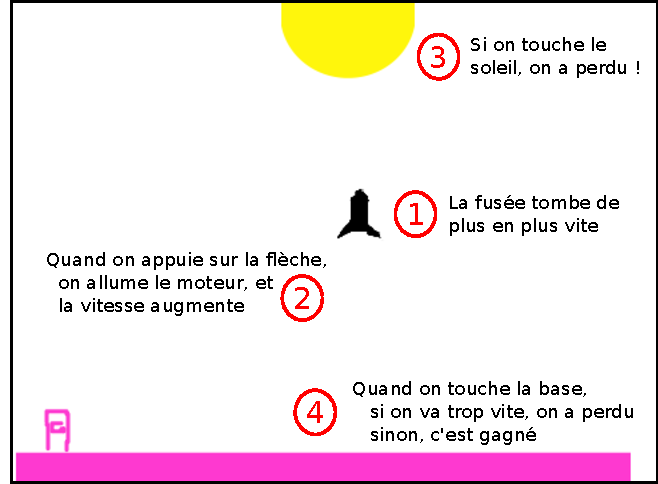
\includegraphics[width=\textwidth]{img/fusee_but-du-jeu.pdf}

\medskip%
\centerline{Premier jeu à faire en \snap{} (ou Scratch)}
  
\vfill%\smallskip
\begin{center}
\begin{spacing}{.8}
  \centerline{\footnotesize Télécharge ce livret, et d'autres activités sur}

  \centerline{\small\color{blue}\url{http://www.loria.fr/~quinson/C4K}}
\end{spacing}

\vspace{.2\baselineskip}
\begin{minipage}{.8\linewidth}
  \begin{spacing}{.5}
    \hbox to \linewidth{\tiny~\hfill Vous pouvez copier, modifier et diffuser librement ce document,}
    \hbox to \linewidth{\tiny~\hfill à la seule condition de laisser ces mêmes droits à vos lecteurs.}
  \end{spacing}
\end{minipage}%
~
\begin{minipage}[b]{.16\linewidth}
  
\includegraphics[width=\linewidth]{img/logo_by-sa.pdf}
\end{minipage}%
\end{center}


%%%%%%%%%%%%%%%%%%%%%%%%%%%%%%%%%%%%%%%%%%%%%%%%%%%%%%%%%%%%%%%%%%%%%%%%%%%%
%%%%%%%%%%%%%%%%%%%%%%%%%%%%%%%%%%%%%%%%%%%%%%%%%%%%%%%%%%%%%%%%%%%%%%%%%%%%
%%%%%%%%%%%%%%%%%%%%%%%%%%%%%%%%%%%%%%%%%%%%%%%%%%%%%%%%%%%%%%%%%%%%%%%%%%%%
\newpage 
\section*{Principe du jeu}

\vspace{-.5\baselineskip}
On doit poser sa fusée sans la scratcher.

Si on appuie sur \textit{espace}, le moteur la fait accélérer vers le haut.
%
Si on ne fait rien, elle tombe (de plus en plus vite). 

On a gagné si on arrive tout doucement sur la base. On a perdu si on se pose
trop vite, ou si on touche le soleil.

\vspace{-.5\baselineskip}
\section*{Il te faut trois lutins}
\vspace{-.5\baselineskip}
\centerline{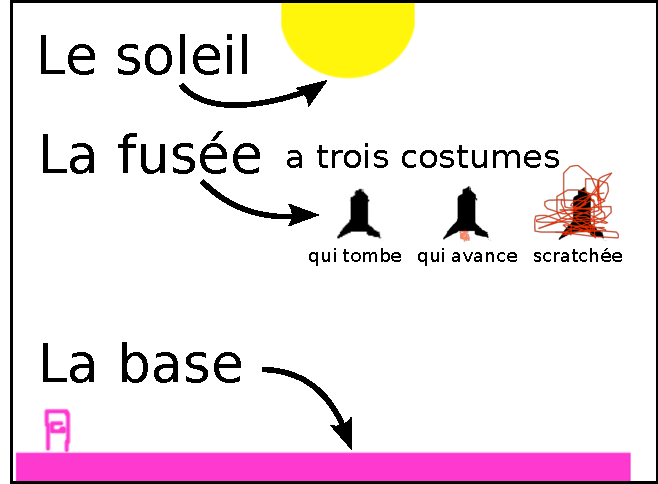
\includegraphics[width=.8\linewidth]{img/fusee_lutins.pdf}}

\bigskip
\centerline{\it Comment créer ces lutins?}

%%%%%%%%%%%%%%%%%%%%%%%%%%%%%%%%%%%%%%%%%%%%%%%%%%%%%%%%%%%%%%%%%%%%%%%%%%%% 
%%%%%%%%%%%%%%%%%%%%%%%%%%%%%%%%%%%%%%%%%%%%%%%%%%%%%%%%%%%%%%%%%%%%%%%%%%%%
%%%%%%%%%%%%%%%%%%%%%%%%%%%%%%%%%%%%%%%%%%%%%%%%%%%%%%%%%%%%%%%%%%%%%%%%%%%%
\newpage
\section*{Qu'est ce qu'un lutin?}
Les lutins sont des dessins à l'écran que l'on peut commander en écrivant des
scripts.
\medskip

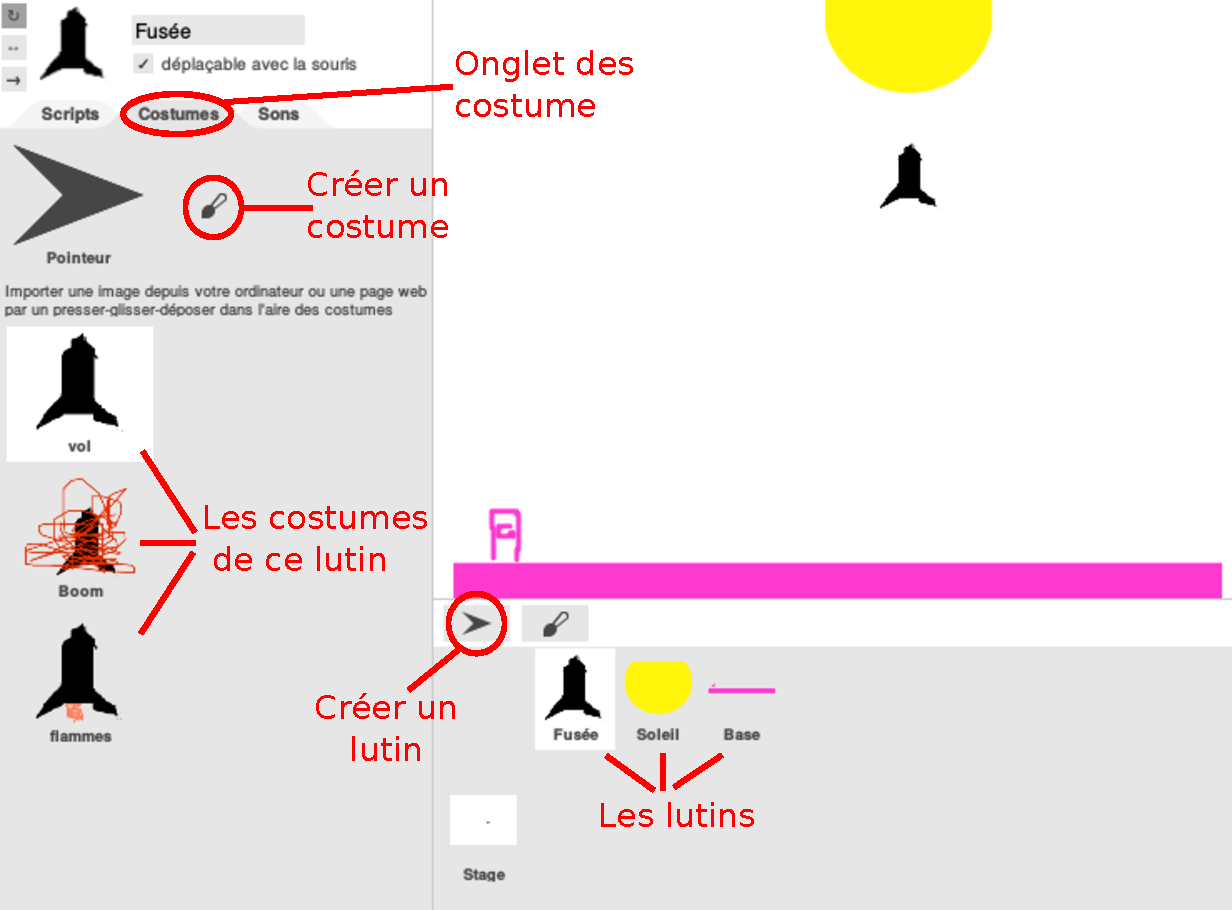
\includegraphics[width=\linewidth]{img/snap-costume.pdf}

\bigskip%
Crée tes lutins, puis dessine leurs costumes.

\bigskip
\bigskip
\centerline{\it Comment faire bouger mes lutins?}

%%%%%%%%%%%%%%%%%%%%%%%%%%%%%%%%%%%%%%%%%%%%%%%%%%%%%%%%%%%%%%%%%%%%%%%%%%%%
%%%%%%%%%%%%%%%%%%%%%%%%%%%%%%%%%%%%%%%%%%%%%%%%%%%%%%%%%%%%%%%%%%%%%%%%%%%%
%%%%%%%%%%%%%%%%%%%%%%%%%%%%%%%%%%%%%%%%%%%%%%%%%%%%%%%%%%%%%%%%%%%%%%%%%%%%
\newpage
\section*{Qu'est ce qu'un script?}
\vspace{-.7\baselineskip}
Les briques sont des ordres que le lutin comprend.
%
Elles sont triées par couleur:

\centerline{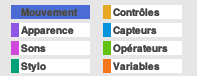
\includegraphics[width=.65\linewidth]{img/snap-categories.png}}

Il y a beaucoup de briques possibles, mais heureusement, on en utilise peu à la
fois!
%
Essaye de combiner les briques suivantes:


\includegraphics[scale=.45]{img/snap-avance.png}\hfill

\includegraphics[scale=.45]{img/snap-bump.png}

\vspace{-.2\baselineskip}

\includegraphics[scale=.45]{img/snap-hello.png}\hfill

\includegraphics[scale=.45]{img/snap-tourne.png}

\vspace{-.2\baselineskip}

\includegraphics[scale=.45]{img/snap-size.png}\hfill

\includegraphics[scale=.45]{img/snap-sleep.png}

\vspace{-.2\baselineskip}
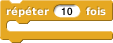
\includegraphics[scale=.45]{img/snap-repete.png}\hfill

\includegraphics[scale=.45]{img/snap-click.png}

\vspace{-.7\baselineskip}
\section*{Faire descendre la fusée}
\vspace{-.7\baselineskip}

\begin{minipage}{.6\linewidth}
  Il est temps de faire notre premier vrai script, puis de cliquer dessus.
\end{minipage}\hfill
\begin{minipage}{.35\linewidth}
  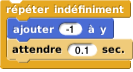
\includegraphics[scale=.5]{img/fusee_vitesse-cste.png}
\end{minipage}

\medskip
\centerline{\it Mince, j'ai perdu la fusée (en bas)!}

%%%%%%%%%%%%%%%%%%%%%%%%%%%%%%%%%%%%%%%%%%%%%%%%%%%%%%%%%%%%%%%%%%%%%%%%%%%%
%%%%%%%%%%%%%%%%%%%%%%%%%%%%%%%%%%%%%%%%%%%%%%%%%%%%%%%%%%%%%%%%%%%%%%%%%%%%
%%%%%%%%%%%%%%%%%%%%%%%%%%%%%%%%%%%%%%%%%%%%%%%%%%%%%%%%%%%%%%%%%%%%%%%%%%%%
\newpage

\section*{Ne plus perdre la fusée}
\vspace{-.8\baselineskip}

\begin{minipage}[b]{.53\linewidth}
  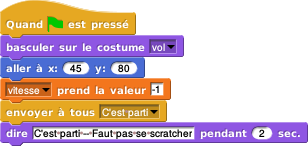
\includegraphics[scale=.5]{img/fusee_init.png}
\end{minipage}
\begin{minipage}[b]{.48\linewidth}
  \hspace{-2.5mm}On revient au départ.

  On note que la \\ 
  \null~~vitesse est -1.

  On déclenche les \\ 
  \null~~autres scripts.

  \vspace{.3\baselineskip}~
\end{minipage}


\begin{minipage}{.53\linewidth}
  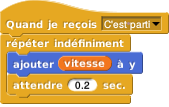
\includegraphics[scale=.5]{img/fusee_descendre.png}
\end{minipage}
\begin{minipage}{.47\linewidth}
  Quand ça démarre, on descend comme avant.
\end{minipage}

La fusée a maintenant deux scripts.

\vspace{-.8\baselineskip}
\section*{Tomber toujours plus vite}
\vspace{-.8\baselineskip}

\begin{minipage}{.5\linewidth}
  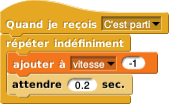
\includegraphics[scale=.5]{img/fusee_tomber-plus-vite.png}
\end{minipage}
\begin{minipage}{.5\linewidth}
  Ce troisième script de la fusée change régulièrement la\\ vitesse.
\end{minipage}

Si la fusée glisse mollement ou se précipite au sol, corrige les délais et la
vitesse.

%%%%%%%%%%%%%%%%%%%%%%%%%%%%%%%%%%%%%%%%%%%%%%%%%%%%%%%%%%%%%%%%%%%%%%%%%%%% 
%%%%%%%%%%%%%%%%%%%%%%%%%%%%%%%%%%%%%%%%%%%%%%%%%%%%%%%%%%%%%%%%%%%%%%%%%%%%
%%%%%%%%%%%%%%%%%%%%%%%%%%%%%%%%%%%%%%%%%%%%%%%%%%%%%%%%%%%%%%%%%%%%%%%%%%%%
\newpage
\section*{Le moteur fait remonter}
\vspace{-.7\baselineskip}

Un quatrième script ajoute de la vitesse vers le haut quand on active le moteur.

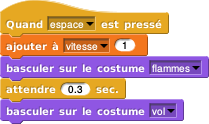
\includegraphics[scale=.5]{img/fusee_moteur.png}

\section*{Ne touche pas le soleil!}
\vspace{-.7\baselineskip} %
Pour détecter si la fusée se brûle dans le soleil, il faut ajouter un cinquième
script qui bloque jusqu'au moment du contact.

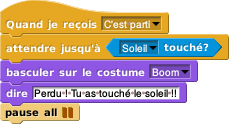
\includegraphics[scale=.5]{img/fusee_fin-soleil.png}

%\medskip
%\centerline{\it Comment utiliser avec le moteur?}


%%%%%%%%%%%%%%%%%%%%%%%%%%%%%%%%%%%%%%%%%%%%%%%%%%%%%%%%%%%%%%%%%%%%%%%%%%%% 
%%%%%%%%%%%%%%%%%%%%%%%%%%%%%%%%%%%%%%%%%%%%%%%%%%%%%%%%%%%%%%%%%%%%%%%%%%%%
%%%%%%%%%%%%%%%%%%%%%%%%%%%%%%%%%%%%%%%%%%%%%%%%%%%%%%%%%%%%%%%%%%%%%%%%%%%%
\newpage
\section*{Toucher la base}
\vspace{-.7\baselineskip}


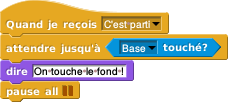
\includegraphics[scale=.5]{img/fusee_touche-fond.png}

\vspace{-.7\baselineskip}
\section*{Posée ou scratchée?}
\vspace{-.7\baselineskip}
gagné ou perdu? 
Ça dépend de la vitesse!

\begin{minipage}{.65\linewidth}
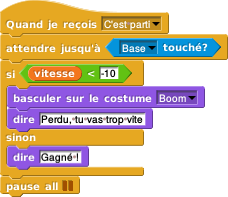
\includegraphics[scale=.5]{img/fusee_fin-base.png}
\end{minipage}
\begin{minipage}{.34\linewidth}
  \small (nouvelle \\
  version du\\ 
  dernier script)
\end{minipage}
\section*{Ton jeu est prêt!!}
\vspace{-.7\baselineskip}
Amuse-toi bien!

%%%%%%%%%%%%%%%%%%%%%%%%%%%%%%%%%%%%%%%%%%%%%%%%%%%%%%%%%%%%%%%%%%%%%%%%%%%% 
%%%%%%%%%%%%%%%%%%%%%%%%%%%%%%%%%%%%%%%%%%%%%%%%%%%%%%%%%%%%%%%%%%%%%%%%%%%%
%%%%%%%%%%%%%%%%%%%%%%%%%%%%%%%%%%%%%%%%%%%%%%%%%%%%%%%%%%%%%%%%%%%%%%%%%%%%
\newpage 
\section*{C'est ton jeu}
\vspace{-.5\baselineskip}

Ce livret t'apprend à fabriquer ton \\
premier jeu en \snap, étape après étape.

\medskip
Quand il est terminé, joue avec tes copains et fais-le évoluer comme tu le
désires.

\vspace{-.3\baselineskip}
\subsection*{Bonus possibles}
\vspace{-.5\baselineskip}

{\it Un chronomètre\hfill Un réservoir d'essence

\smallskip
\centerline{Le soleil change de taille}

\smallskip
Un second niveau, où on tombe plus vite

\smallskip
\centerline{Pouvoir aller à droite et à gauche}

\smallskip
Viser la base\hfill Ramasser des choses

\smallskip
\centerline{Éviter des méchants}

\smallskip
\begin{minipage}{.5\linewidth}
  \center
  Changer la fusée\\
  en sous-marin
\end{minipage}%
\begin{minipage}{.5\linewidth}
  \center
  Changer la fusée\\
  en hélicoptère
\end{minipage}
}

\vspace{-.3\baselineskip}
\subsection*{Savoir programmer permet}
\vspace{-.7\baselineskip} %
de créer des choses auxquelles personne n'avait pensé. Profites-en pour
inventer!

\end{document}
